\section{Introduction}
In the present article, we replicate the results of Huisman \& Weissing 1999 ``Biodiversity of plankton by species oscillations and chaos'' \cite{1999:Huisman}, an attempt to resolve the paradox of 
the plankton \cite{1961:Hutchinson} with a nonlinear ordinary differential equations model based on resource competition theory.\\

According to many mathematical models, the number of phytoplankton species in a single homogeneous medium cannot exceed the number of separate resources available \cite{1960:Hardin,1973:Phillips,1980:Armstrong}. However it is very common to observe more species than easily identifiable resources in field conditions. This led Hutchinson to formulate the paradox of the plankton \cite{1961:Hutchinson}. Using numerical simulations of their ODE model, Huisman \& Weissing \cite{1999:Huisman} showed that ``supersaturated coexistence'' is possible, where more consumer species than resource items coexist through oscillations or chaos. We attempt here to check this finding. \\

In addition to the replication of the numerical results of Huisman and Weissing \cite{1999:Huisman}, we also present two novel numerical experiments inspired by follow-up articles, ``Does ``supersaturated coexistence'' resolve the ``paradox of the plankton'' ?'' by Schippers et al. 2008 \cite{2008:Schippers}, and ``Towards a solution of the plankton paradox: the importance of physiology and life history'' by Huisman et al. 2008 \cite{2008:Huisman}. These articles suggested that supersaturated coexistence might be difficult to obtain outside of the restricted parameter scenarios considered in the original article. Schippers et al. \cite{2008:Schippers} perturbed parameters mostly species by species to show model sensitivity to parameters, concluding that supersaturated coexistence was unlikely, while Huisman et al. \cite{2008:Huisman} show how some trade-offs can make parameter combinations favourable to coexistence emerge (although most of the scenarios they consider confirm the results of Schippers et al. \cite{2008:Schippers}). Here we further consider mild perturbation of intrinsic growth rates of all species at once (though not necessarily in the same direction), an hypothesis which we deem coherent with whole-ecosystem perturbations. If supersaturated coexistence is a likely coexistence mechanism, small changes to growth rates should not massively affect the number of coexisting species. 

\section{Model}

We describe below the model of phytoplankton community dynamics of Huisman \& Weissing \cite{1999:Huisman}. Let $N_i$ and $R_j$ respectively be the population density of species $i$ and concentration of resource $j$, $i\in[\![1,n]\!]$ and $j\in[\![1,k]\!]$ with $n$ and $k$ the number of different species and resources. The time derivatives of $N_i$ and $R_j$ are given by: \\

\begin{align}
	& \frac{dN_i}{dt}= N_i(\mu_i(R_1,...,R_k)~-~m_i)\\
	& \frac{dR_j}{dt}= D(S_j-R_j) - \sum_{i=1}^n c_{ji} 
\mu_i(R_1,...,R_k)N_i
\end{align}

with parameters

\begin{align*}
& m_i \text{ the mortality rate of species $i$}\\
& D \text{ the system's turnover rate}\\
& S_j \text{ the supply concentration of resource $j$}\\
& c_{ji} \text{ the content of resource $j$ in species $i$}\\
& \mu_i \text{ the growth rate of species $i$, defined using the Monod equation and Liebig's law of minimum: }
\end{align*}

\begin{align}
&\mu_i(R_1,...,R_k)~=~\min_{j\in[\![1,k]\!]} \left( \frac{r_iR_j}{K_{ji}+R_j} \right). 
\end{align}

The growth rates are defined using: 
\begin{align*}
&r_i \text{ the maximum growth rate of species $i$}\\
&K_{	ji} \text{ the half-saturation constant for resource $j$ of species $i$.}
\end{align*}

In order to reproduce the results of Huisman \& Weissing \cite{1999:Huisman}, the differential equations were integrated using the \texttt{deSolve} package in its 1.32 version in \texttt{R} 4.2.0, using the same parameter sets as in the original article.\\

Multiple simulations are performed and illustrated in the original article as well as here: \\
In Figure \ref{figures:Fig1} a) and b), 3 species are competing for 3 resources, in c), 6 species are competing for 3 resources and in d), 9 species are competing for 3 resources. In Figure \ref{figures:Fig2}, 5 species are competing on 3 resources. In Figure \ref{figures:Fig3}, 5 species are competing on 5 resources. In Figure \ref{figures:Fig4}, 12 species are competing for 5 resources. 
In Figure \ref{figures:Fig2} and Figure \ref{figures:Fig1} a), b) and for the 
bifurcation diagram of Figure \ref{figures:Fig3}, all of the species are 
introduced at the same time in the simulation. In Figure \ref{figures:Fig4} and 
Figure \ref{figures:Fig1} c), d), the species were introduced sequentially. 
Huisman et al. \cite{1999:Huisman} have provided the starting times 
of each species introductions when needed, in addition to the dynamical parameters.\\


As Schippers et al. \cite{2008:Schippers}, we were wondering how and why the parameter sets were initially chosen, 
and if the results would remain the same for slightly different parameters. Several simulations were made in 
Schippers et al. paper \cite{2008:Schippers} and Huisman et al.'s response\cite{2008:Huisman}, in order to evaluate how robust was supersaturated 
coexistence. In the same spirit, we carried out new numerical experiments with a slightly different perspective.\\

We chose to focus on evaluating the robustness of the last simulation of Huisman \& Weissing \cite{1999:Huisman}, displayed on Figure \ref{figures:Fig4}. We focused on perturbating the growth rate parameter, $r_i$, denoted as $\mu_{\text{max}}$ in the follow-up articles \cite{2008:Schippers,2008:Huisman}. 
As changing only a single one of the $n$ intrinsic growth rates $r_i$ (as done earlier in the follow-up articles \cite{2008:Schippers,2008:Huisman}) appeared a little artificial to us, 
we chose to randomly perturb all of the $n~~r_i$ at once, as would typically do an ecosystem-wide perturbation that is not directly related to the modelled resources. 
In a first numerical experiment, we considered the exact same invasion sequence as Huisman \& Weissing \cite{1999:Huisman}. 
In a second step, we started with the full set of species at once.\\
\\
In order to conduct the numerical experiments proposed earlier, the method used to plot the 
fourth Figure has been reused. The two experiments were conducted 400 times each, 
with as many different parameter sets: the $r_i$ were drawn according to a 
truncated normal distribution. The mean was $\mu=1$ and the variance was 
$\sigma=0.1$, corresponding to CV=10\%. The distribution was truncated using $\mu\pm3\sigma$, in other 
words between $0.7$ and $1.3$.\\~\\ 

\section{Results}

\subsection{Reproduction}

We were able to replicate the four figures of Huisman \& Weissing\cite{1999:Huisman}, presented below. 

\begin{figure}[H]
\begin{center} 
 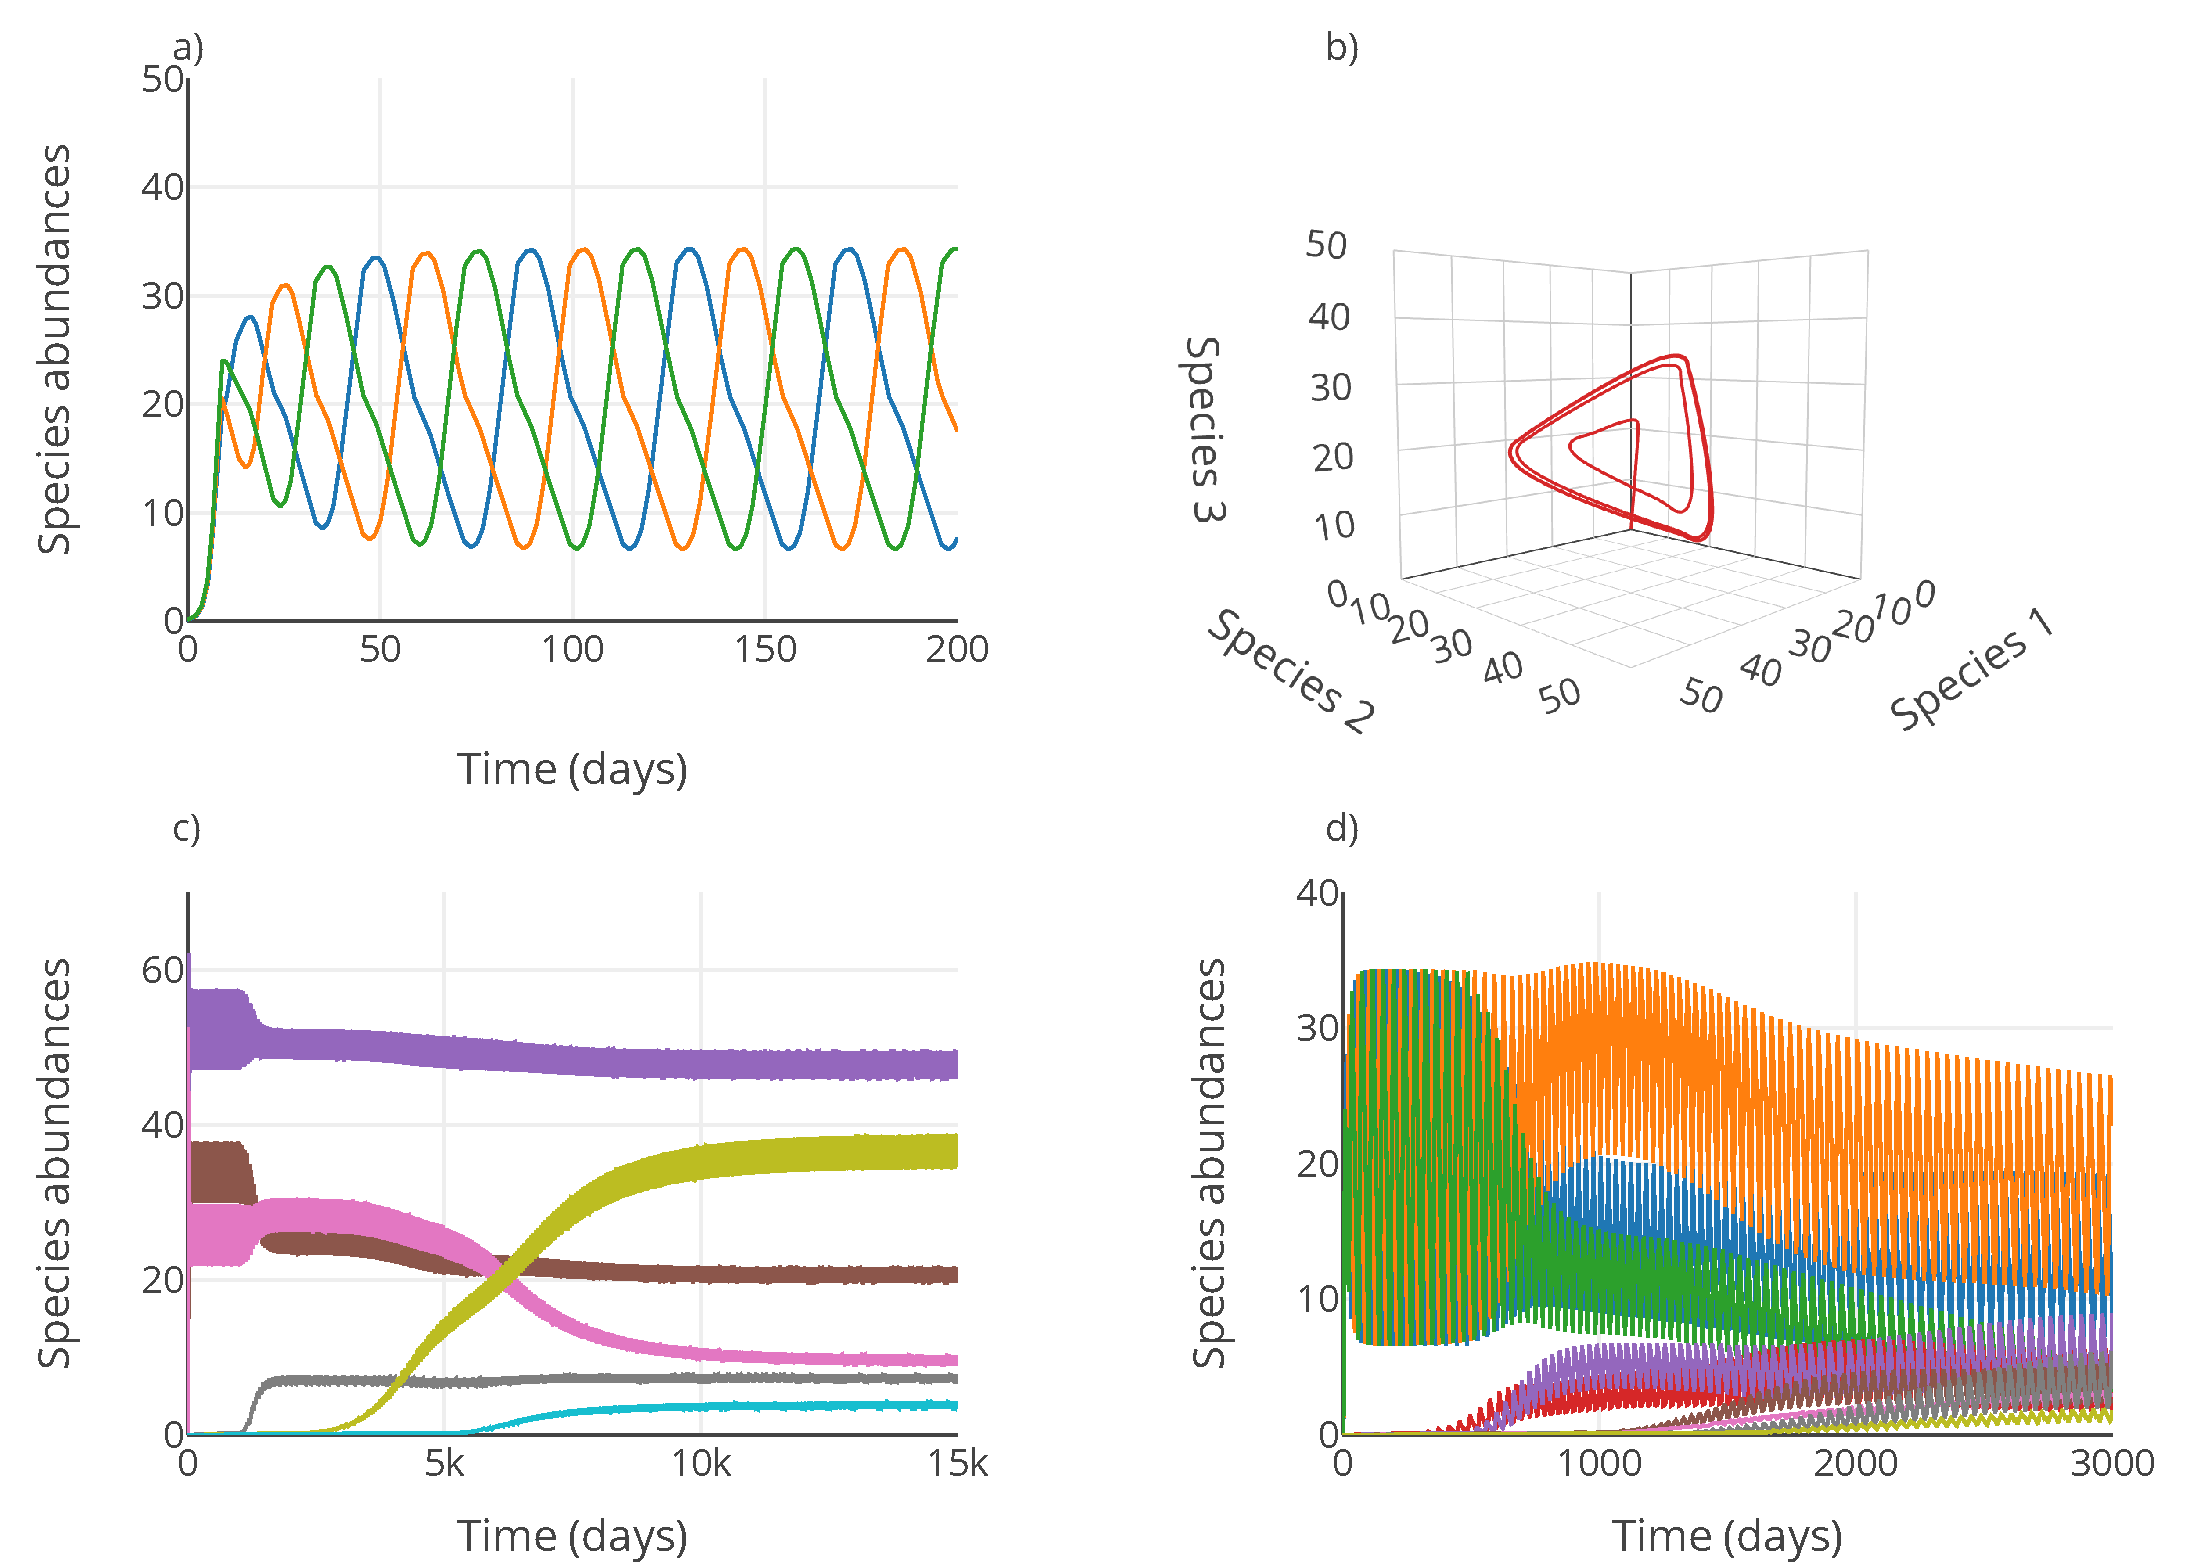
\includegraphics[width=1\textwidth]{../Code/Figures/Figure_1.pdf}
  \caption{Oscillations on three resources. a), Time course of the abundances 
of three species competing for three resources. b), The corresponding limit 
cycle. c), Small-amplitude oscillations of six species on three resources. 
d), Large-amplitude oscillations of nine species on three resources.}
  \label{figures:Fig1}
\end{center}
\end{figure}

\begin{figure}[H]
\begin{center} 
 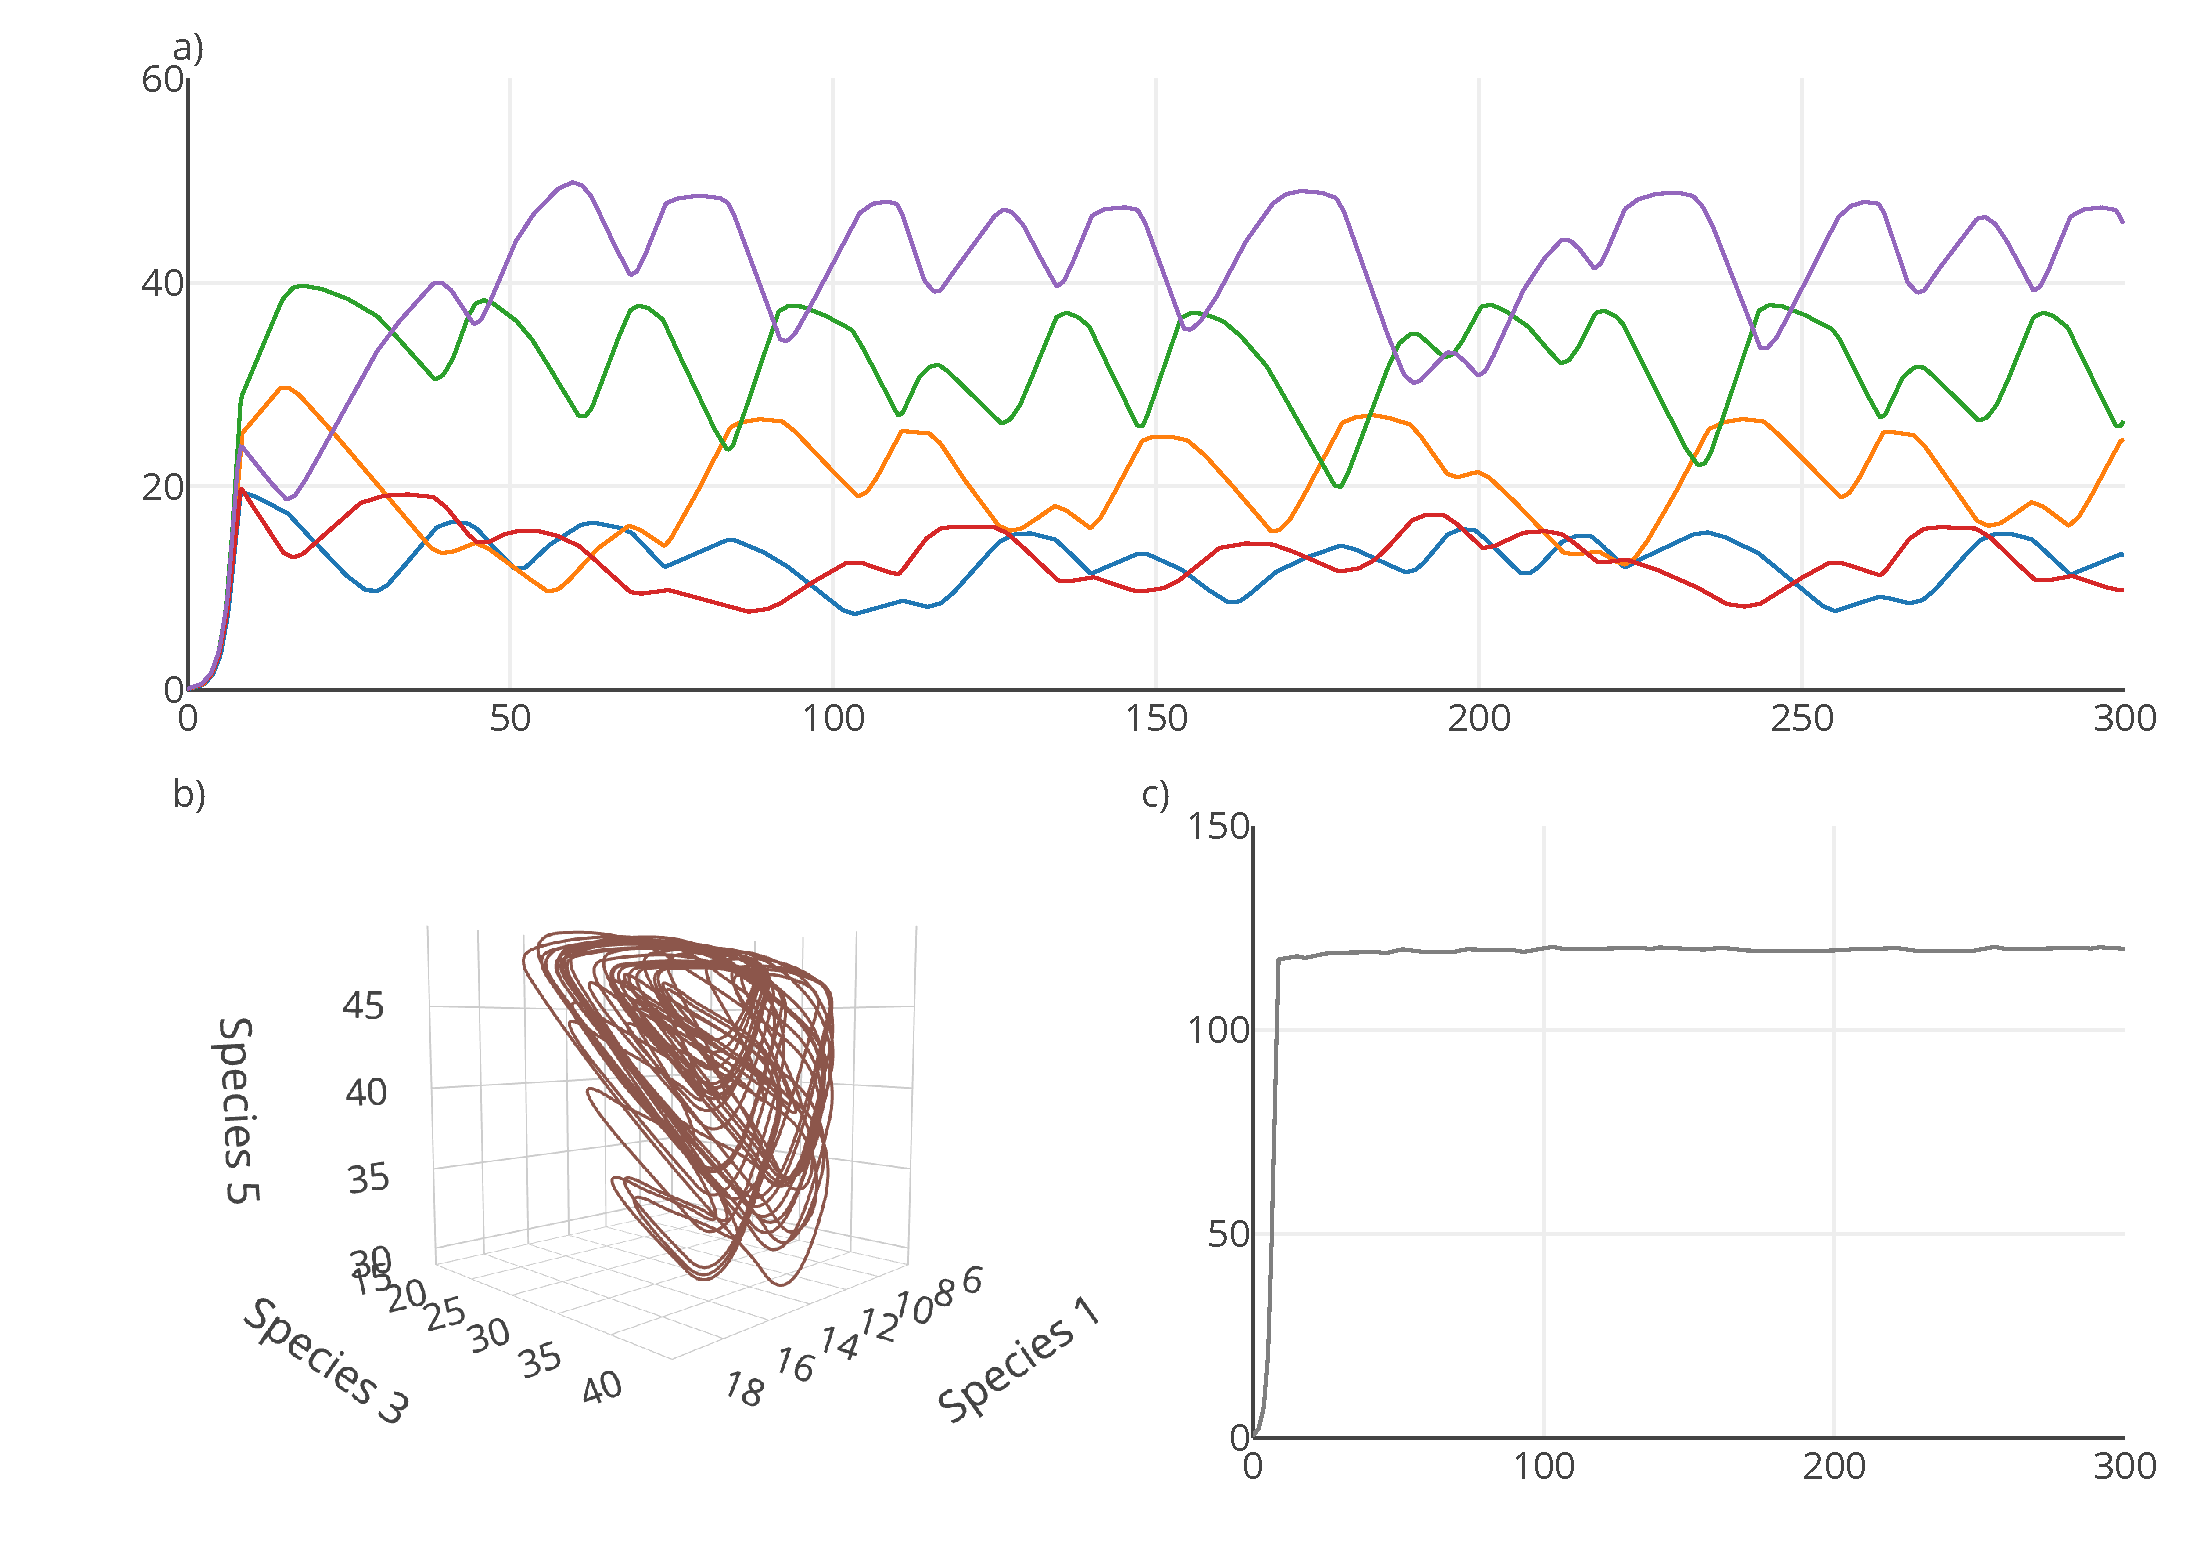
\includegraphics[width=1\textwidth]{../Code/Figures/Figure_2.pdf}
  \caption{Chaos on five resources. a) time course of the abundances of five species competing for five resources, b) corresponding chaotic attractor. The trajectory is plotted for three of the five species, from the period from $t= 1,000$ to $t=2,000$ days, c) time course of total community biomass.}
  \label{figures:Fig2}
\end{center}
\end{figure}

\begin{figure}[H]
\begin{center} 
 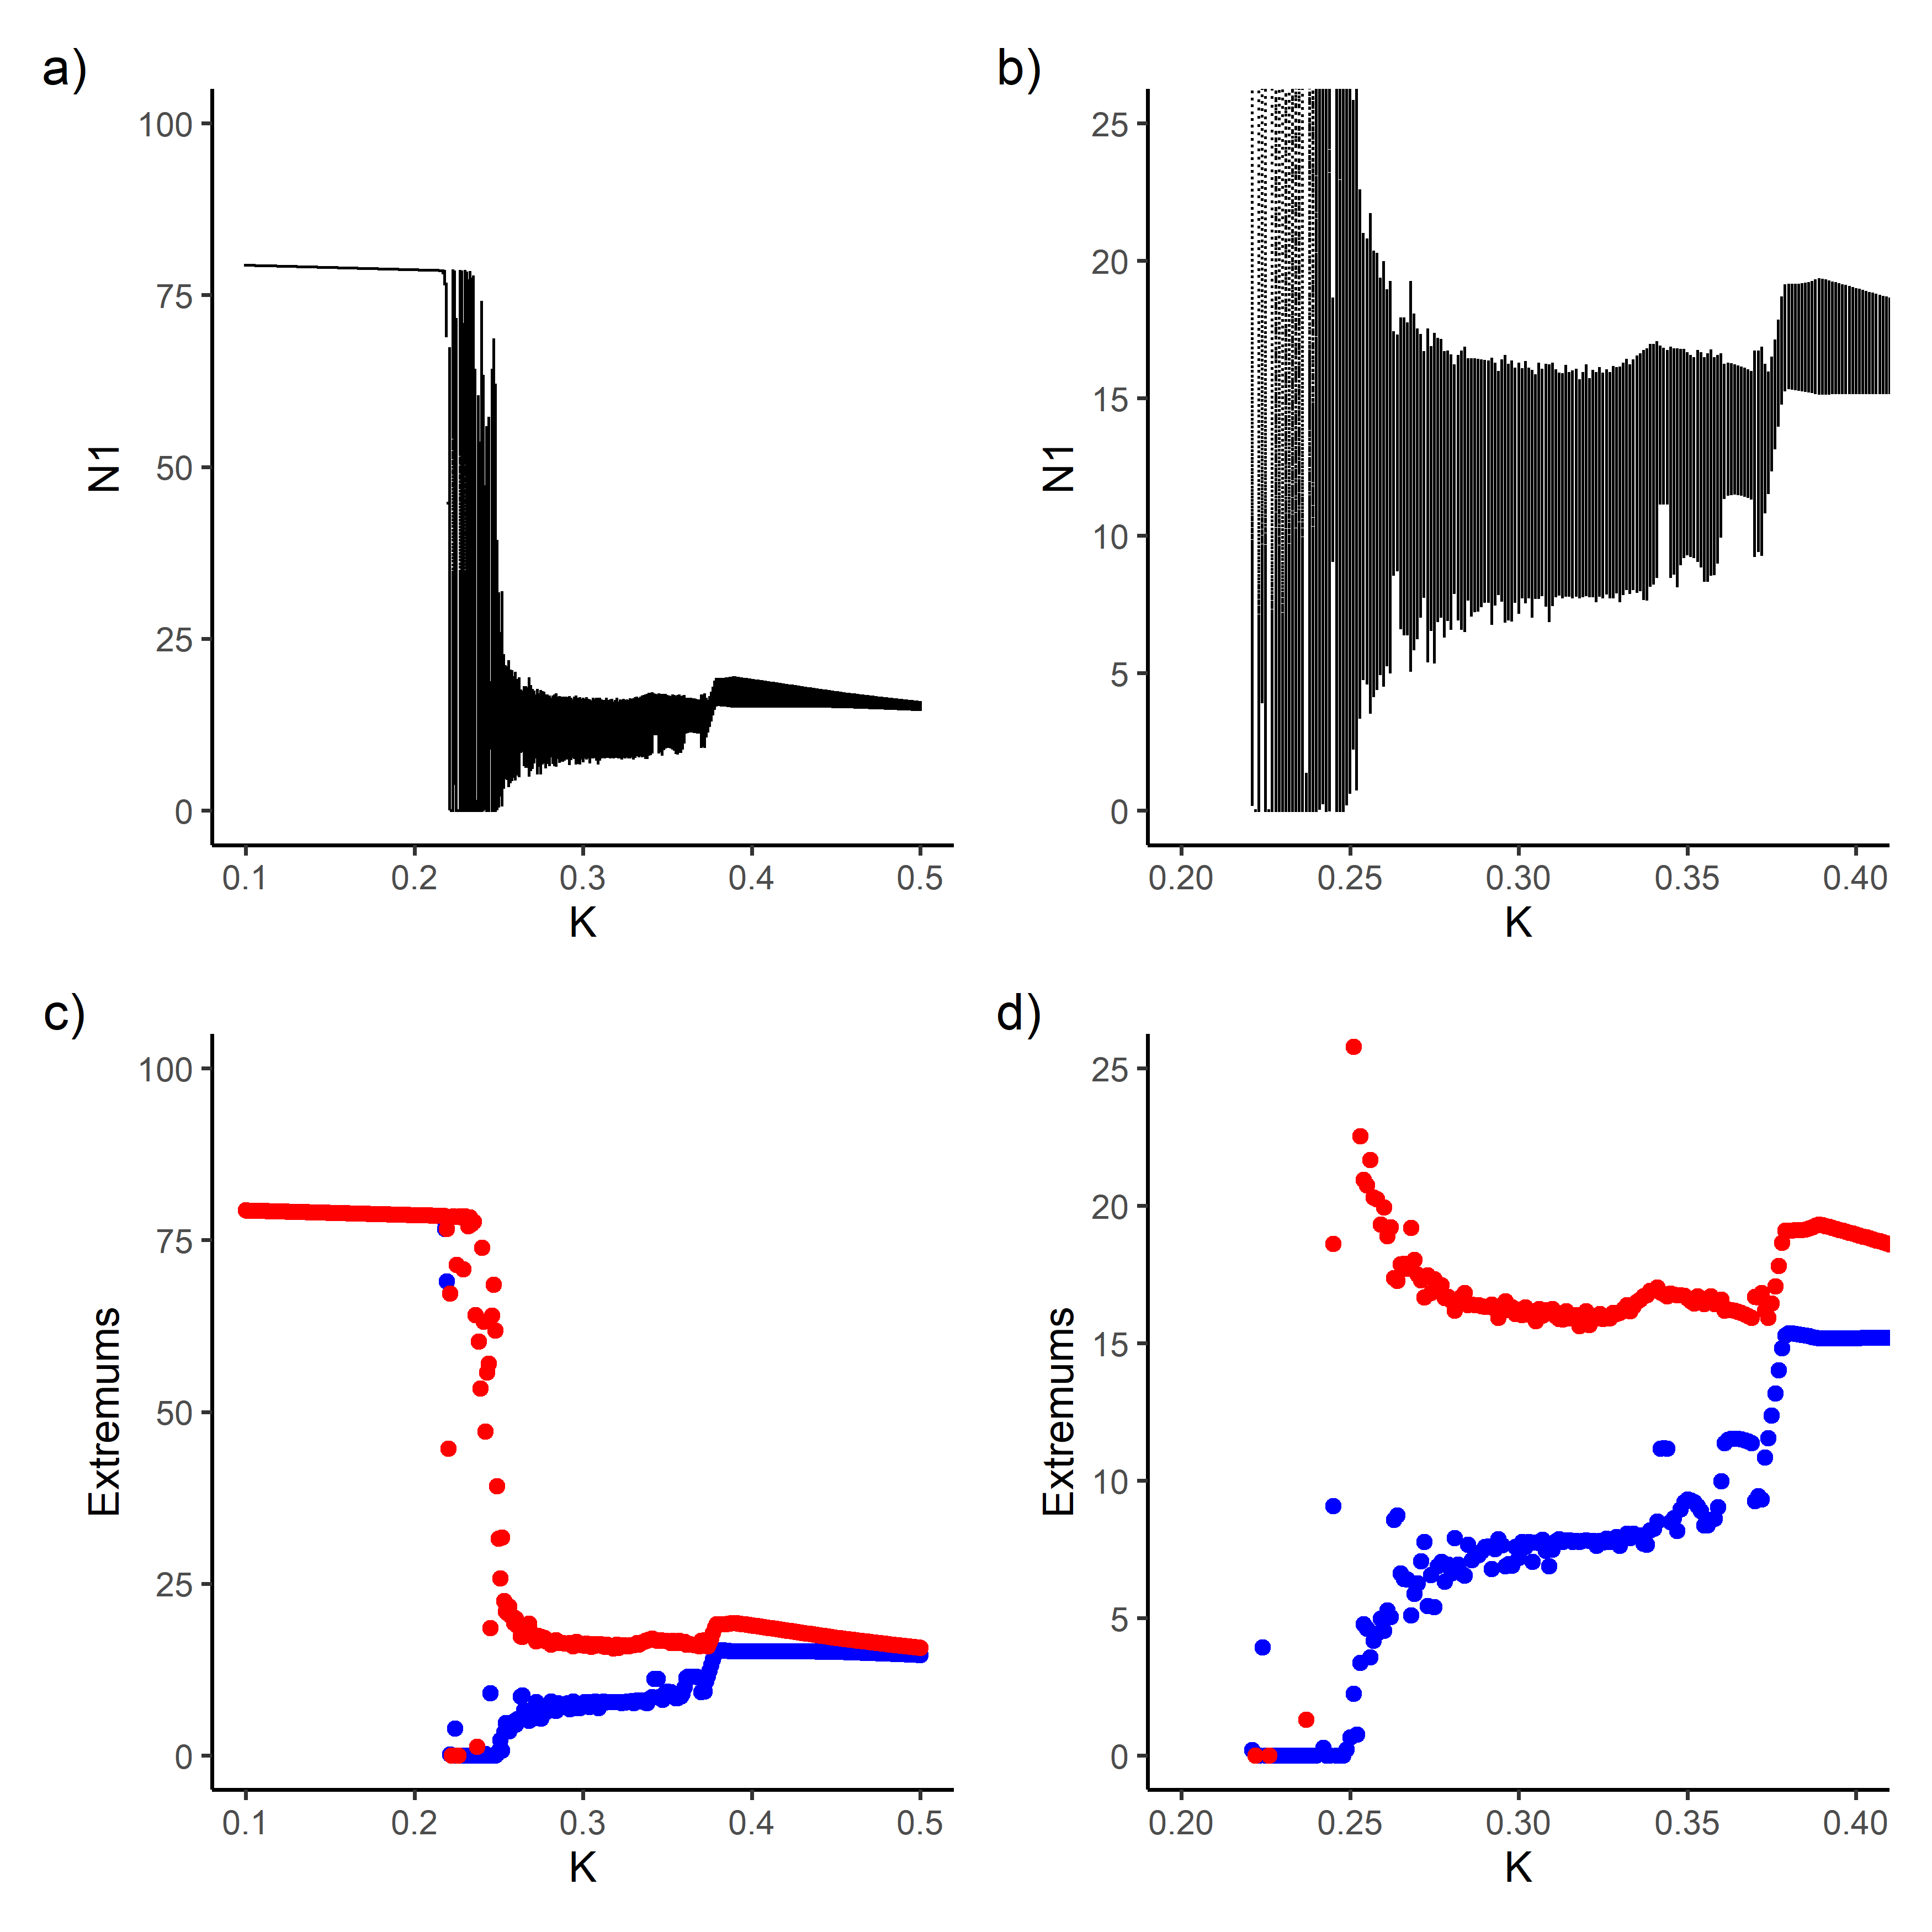
\includegraphics[width=1\textwidth]{../Code/Figures/Figure_3.png}
  \caption{Bifurcation diagram, for five species competing for five resources. a) Show all of the values of species 1, plotted during the period from $t=2,000$ to $t=4,000$ days, as a function of the half-saturation constant $K_{41}$. Part of a) is magnified in b). c) show the local minima and maxima of species 1, plotted during the period from t= 2,000 to t=4,000 days, as a function of the half-saturation constant $K_{41}$. Part of c) is magnified in d).}
  \label{figures:Fig3}
\end{center}
\end{figure}

The bifurcation diagram caption did not seem to correspond to the actual Figure, which seemed to display all of the points of the simulation between 
$t=2,000$ and $t=4,000$ rather that only the local extrema. We have therefore chosen to draw those two options. 

\begin{figure}[H]
\begin{center} 
 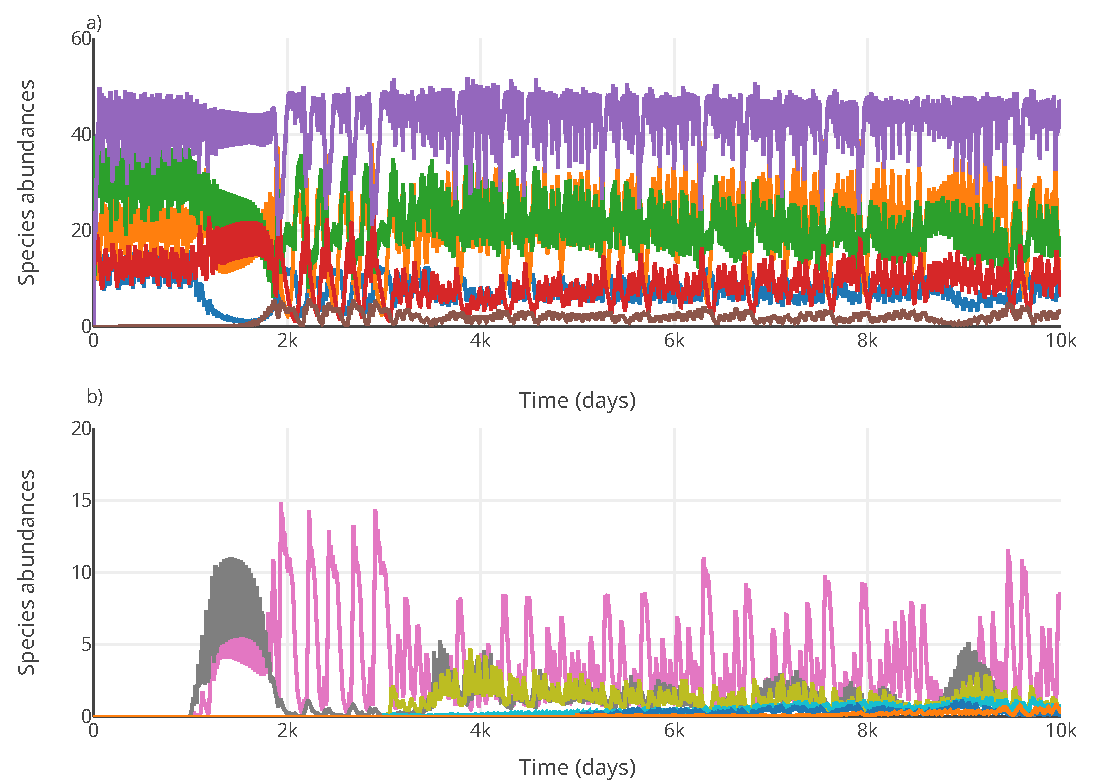
\includegraphics[width=0.86\textwidth]{../Code/Figures/Figure_4.pdf}
  \caption{Competitive chaos and the coexistence of 12 species on five resources. a) abundances of species 1-6, b) abundances of species 7-12.}
  \label{figures:Fig4}
\end{center}
  \end{figure}

\subsection{Experiments}

For the first numerical experiment, introducing species one after the other as in the 
original simulation, the following statistics, displaying the frequencies 
(expressed in \%) of the number of species present at the end of the simulation 
could be obtained: \\
% latex table generated in R 4.2.1 by xtable 1.8-4 package
% Fri Jul 22 17:21:52 2022
\begin{table}[ht]
\centering
\begin{tabular}{rrrrrrrr}
  \hline
 & 0 species & 1 species & 2 species & 3 species & 4 species & 5 species & 6 species \\ 
  \hline
Probability & 0.00 & 13.68 & 26.56 & 35.01 & 11.27 & 8.85 & 4.02 \\ 
   \hline
\end{tabular}
\end{table}

% latex table generated in R 4.2.1 by xtable 1.8-4 package
% Fri Jul 22 17:21:52 2022
\begin{table}[ht]
\centering
\begin{tabular}{rrrrrrrr}
  \hline
 & 7 species & 8 species & 9 species & 10 species & 11 species & 12 species & Supersaturated \\ 
  \hline
Probability & 0.60 & 0.00 & 0.00 & 0.00 & 0.00 & 0.00 & 4.63 \\ 
   \hline
\end{tabular}
\end{table}

\\
A species has been considered present if $N_i > 0.001$ at the end of the simulation. This simulation shows that the persistence of five species or more is very unlikely, and that supersaturated coexistence may be present in a limited domain of parameter space.\\

\\
The pattern of extinction and its interaction for the first experiment is shown in the Figure \ref{figures:Figexp1}. Note that the subfigure 1) represents the original results with $r_i=1 ~\forall i$, while $r_i$ randomly varies as described in the methods for all other panels.

\begin{figure}[H]
\begin{center} 
 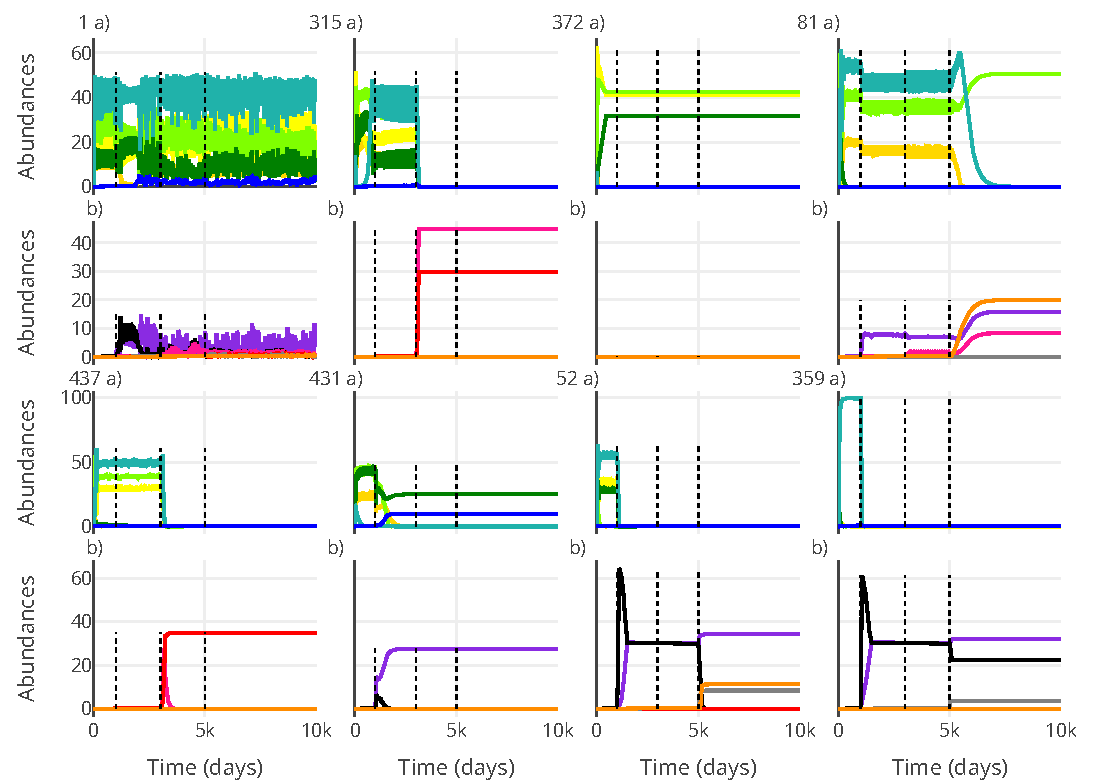
\includegraphics[width=1\textwidth]{../Code/Figures/Figure_exp1.pdf}
  \caption{Visualisation of 8 different simulations of competitive chaos and coexistence of 12 species on five ressources. Identical to Figure 4 except that intrinsic growth rate $r_i$ are randomly varied. Except for the first panel, the simulations illustrated were randomly picked among the 500 constituting the numerical experiment. Each couple of subplots is labelled with the number of the corresponding simulation. a) abundances of species 1-6, b) abundances of species 7-12.}
  \label{figures:Figexp1}
\end{center}
\end{figure}

We observe contrasted stationary endpoints, possibly with some oscillations or chaos during the invasion process. As shown in Figure \ref{figures:Figexp1}, however, most species do not persist. It is also noticable that the 5 species on 5 ressources (before the first invasion at $t=1,000$) is sometimes already unstable.\\
\\
For the second experiment, introducing all species at once, the  following statistics could be obtained, displaying the frequencies (expressed in 
\%) of the number of species present at the end of the simulation :  \\
% latex table generated in R 4.2.1 by xtable 1.8-4 package
% Fri Jul 22 17:21:49 2022
\begin{table}[ht]
\centering
\begin{tabular}{rrrrrrrr}
  \hline
Extant species & 0 & 1 & 2 & 3 & 4 & 5 & 6 \\ 
  \hline
Probability & 0.00 & 36.40 & 41.40 & 5.00 & 10.00 & 6.00 & 1.20 \\ 
   \hline
\end{tabular}
\end{table}

% latex table generated in R 4.2.1 by xtable 1.8-4 package
% Fri Jul 22 17:21:49 2022
\begin{table}[ht]
\centering
\begin{tabular}{rrrrrrrr}
  \hline
 & 7 species & 8 species & 9 species & 10 species & 11 species & 12 species & Supersaturated \\ 
  \hline
Probability & 0.00 & 0.00 & 0.00 & 0.00 & 0.00 & 0.00 & 1.20 \\ 
   \hline
\end{tabular}
\end{table}

\\
(A species has been considered present if $N_i > 0.001$ at the end of the simulation). This simulation shows that the persistence of five species or more is very unlikely and that supersaturated coexistence is consequently very rare in parameter space.\\
\\
The pattern of extinction an its interaction for the second experiment is described in following Figure \ref{figures:Figexp2}, note that the subfigure 1) represent the original results with $r_i=1 ~\forall i$, while $r_i$ randomly varies as described in the methods for all other panels.

\begin{figure}[H]
\begin{center} 
 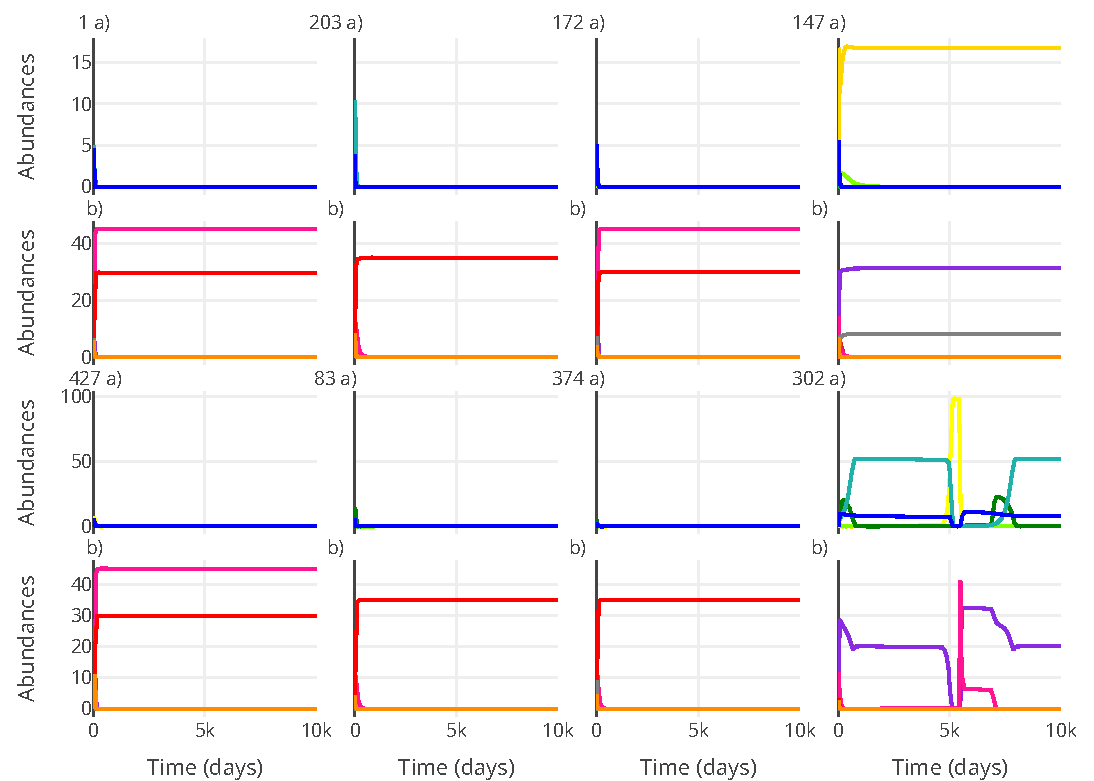
\includegraphics[width=1\textwidth]{../Code/Figures/Figure_exp2.pdf}
  \caption{Visualisation of 8 different simulations of competitive chaos and coexistence of 12 species on five ressources, following the Figure 4 method except that $r_i$ was randomly drawn for each of the species and all species were introduced at once. Except the first panel (original parameters), the simulations illustrated were randomly picked among the 500 of the numerical experiment. Each couple of subplots is labeled with the number of the corresponding simulation. a) abundances of species 1-6, b) abundances of species 7-12.}
  \label{figures:Figexp2}
\end{center}
\end{figure}

As for the first experiment we mostly observed either fixed (non-oscillatory) stationary endpoints or oscillations but with even less persistent species, as shown in Figure \ref{figures:Figexp2}.

\section{Discussion}

We were able to successfully replicate the Figures of the original paper. There are minor differences in species dynamics in Figure~\ref{figures:Fig4}, which are arguably due to differences in numerical integration.\\~\\

The additional numerical experiments showed that slightly changing the values of the $r_i$ parameters almost always prevents the coexistence of 12 species on five ressources and mostly prevents
supersaturated coexistence in general. This is true when introducing species sequentially as in the original paper, as well as all at once. \\~\\

Our results corroborate those of Schippers et al. \cite{2008:Schippers}, who showed that supersaturated coexistence through chaos or oscillations requires peculiar sets of parameters values, which are not robust to small perturbations. Our results, using a slightly different kind of perturbation, are therefore consistent with their conclusion that supersaturated coexistence is unlikely to solve the paradox of the plankton. Additionally, there are other reasons due to mixing and spatial structure, not considered here, which could render supersaturated coexistence unlikely \cite{2008:Roelke}. 



